\documentclass{article}

\usepackage{amsmath}
\usepackage{amssymb}
\usepackage{float}
\usepackage{caption}
\usepackage{ngerman}
\usepackage{float}
\usepackage{tabularx}
\usepackage{makecell}
\usepackage{enumitem}
\usepackage{marvosym}
\setlength{\parindent}{0em}
\begin{document}


\section{Lineare Algebra}

\subsection{Kern, Bild und Rang}

Ein \textbf{Kern} (\(Ker(A)\)) existiert, wenn \(\det(A) = 0\).\\
Der Kern einer Matrix A ist die Lösungsmenge von \(A \cdot \vec{v} = \vec{0}\)\\
\(\rightarrow\) LGS=0 durch elem. Zeilenoperationen lösen.\\

\vspace*{3mm}
Das \textbf{Bild} (\(Im(A)\)) einer Matrix gibt an, welche Menge an Vektoren als Lösungen auftreten können (vgl. Wertebereich bei Funktionen).\\
Das Bild einer Matrix A ist die Lösungsmenge von \(A \cdot \vec{v} = \vec{b}\)\\

\vspace*{3mm}
Der \textbf{Rang} (\(rank(A)\)) einer Matrix A ist die Anzahl der linear unabhängigen Zeilen- bzw. Spaltenvektoren.\\
Der Rang = Anzahl der Nichtnullzeilen der Matrix in Zeilenstufenform.\\
\(\rightarrow\) A durch elem. Zeilenoperationen umformen.\\

\subsection{Determinante}
\begin{figure}[H]
    \begin{equation}
        \det\begin{pmatrix}
        a & b \\
        c & d
        \end{pmatrix}
        = ad - bc
    \end{equation}
    \caption*{2x2 Matrix}
\end{figure}

\begin{figure}[H]
    \begin{equation}
        \det\begin{pmatrix}
        a & b & c \\
        d & e & f \\
        g & h & i
        \end{pmatrix}
        = aei + bfg + cdh - gec - hfa - ibd
    \end{equation}
    \caption*{3x3 Matrix}
\end{figure}

\subsubsection*{Ergänzung: Laplace'scher Entwicklungssatz bei höherrangigen Matrizen}
Siehe: https://www.mathebibel.de/laplace-entwicklungssatz


\subsection{Eigenwerte, Eigenvektoren und Eigenraum}

Eine Zahl \(\lambda\) heißt Eigenwert der Matrix A, wenn es einen Vektor \(\vec{v}\) gibt, der nicht der Nullvektor ist, so dass gilt:

\begin{equation*}
    \begin{split}
        A v &= \lambda v \\
        A v - \lambda v &= 0 \\
        (A - \lambda I) v &= 0
    \end{split}
\end{equation*}


\subsubsection{Charakteristisches Polynom berechnen}
\label{sec:charPolynom}
Anstatt o.g. Gleichung zu lösen: Bestimmung der Nullstellen des charakteristischen Polynoms \(p_A(\lambda)\) der Matrix A.

\begin{equation*}
    \begin{split}
    p_A(\lambda) & = \det(A - \lambda I) \\
    & = \begin{vmatrix}
    a_{11} - \lambda & \cdots & a_{1n} \\
    \vdots & \ddots & \vdots \\
    a_{n1} & \cdots & a_{nn} - \lambda
    \end{vmatrix} \overset{!}{=} 0
    \end{split}
\end{equation*}

\subsubsection{Eigenvektoren berechnen}
Der zu einem Eigenwert \(\lambda_i\) gehörende Eigenvektor \(\vec{v_i}\) ist die Lösung der Gleichung:

\begin{equation*}
    \begin{split}
        A\vec{v_i} &= \lambda_i \vec{v_i} \\
        (A - \lambda_i I) \cdot \vec{v_i} &= \vec{0}
    \end{split}
\end{equation*}

\textit{Rechenweg:}

\begin{enumerate}
    \item \(\lambda_i\) für \(\lambda\) in die Matrix \((A-\lambda I)\) einsetzen (siehe charakterisches Polynom)
    \item Das folgende LGS durch elementare Zeilenoperationen lösen:\\
        \begin{equation*}
            \left( 
            \begin{array}{ccc|c}
                a_{11} - \lambda & \cdots & a_{1n} & 0\\
                \vdots & \ddots & \vdots & 0\\
                a_{n1} & \cdots & a_{nn} - \lambda & 0
            \end{array}
            \right)
        \end{equation*}
    \item Für Nullzeilen ergeben sich beliebige Lösungen, die gleich 1 gesetzt werden können.
\end{enumerate}


\subsubsection{Eigenraum berechnen}

Der Eigenraum \(E_A(\lambda_i)\) einer Matrix A zu einem Eigenwert \(\lambda_i\) ist die Menge aller Eigenvektoren \(\vec{v_i}\) zu \(\lambda_i\).\\

\textit{Lösung:}
Vielfaches der Eigenvektoren in Mengenschreibweise festhalten:\\

\begin{equation*}
    E_A(\lambda_i) = \{ k \cdot \vec{v_i} | k \in \mathbb{R} \}   
\end{equation*}

\subsubsection{algebraische vs. geometrische Vielfachheit von \(\lambda\)}
\begin{itemize}
    \item \textbf{algebraische Vielfachheit}: Anzahl gleicher Eigenwerte im charakteristischen Polynom; \(\leq dim(A)\)
    \item \textbf{geometrische Vielfachheit}: Dimension (Anzahl der Vektoren) des Eigenraums \(E(\lambda)\); \(\leq\) algebraische Vielfachheit
\end{itemize}

\(\rightarrow\) Wenn algebraische Vielfachheit = geometrische Vielfachheit, dann ist die Matrix diagonalisierbar.

\subsection{Orthogonale Matrizen}

Zwei Vektoren sind orthogonal, wenn ihr \textbf{Skalarprodukt}\\ 
\begin{equation*}
    \langle a, b \rangle = a_1 b_1 + \hdots + a_i b_i\ = 0
\end{equation*}

\underline{Äquivalente Aussagen:}
\begin{itemize}
    \item Matrix \(B\) ist orthogonal
    \item \(B^T B = I\), d.h. \(B\) ist invertierbar mit \(B^{-1}=B^T\).
    \item Die Spaltenvektoren von B definieren eine Orthonomalbasis von \(\mathbb{R}^n\)\\
\end{itemize}

\subsubsection{Orthogonalen Vektor mit dem Kreuzprodukt finden}
Für \(\vec{a} \bot \vec{b}\) ergibt sich \(\vec{c}\) mit \(\vec{c} \bot \vec{a}\text{ und }\vec{c} \bot \vec{b}\) aus:
\begin{equation*}
    \vec{c} = 
    \vec{a} \times \vec{b} = \begin{pmatrix}
        a_1 \\
        a_2 \\
        a_3
    \end{pmatrix} \times
    \begin{pmatrix}
        b_1 \\
        b_2 \\
        b_3
    \end{pmatrix} =
    \begin{pmatrix}
        a_2 b_3 - a_3 b_2 \\
        a_3 b_1 - a_1 b_3 \\
        a_1 b_2 - a_2 b_1
    \end{pmatrix}
\end{equation*}

\subsubsection{Projektion eines Punktes auf eine Gerade}

Gegeben: Punkt \(P\) und Gerade \(g\) durch den Ursprung \((0,0)\) mit Richtungsvektor \(\vec{r}\). Dann berechnet sich die Projektion von \(P\) auf \(g\) wie folgt:

\begin{equation*}
    \vec{p} = \frac{\langle \vec{p}, \vec{r} \rangle}{||\vec{r}||^2} \vec{r} \text{  bzw. wenn } ||\vec{r}||=1 \text{ dann } \vec{p} = \langle \vec{p}, \vec{r} \rangle \vec{r}
\end{equation*}

\subsubsection{Gram-Schmidt-Verfahren}
\textit{Ziel:} Orthonormalbasis (ONB) zu einem Vektorraum \(B=\{b_1, b_2, \hdots b_n\}\) finden.

\begin{enumerate}
    \item Ersten Basisvektor normieren: \(\vec{q_1} = \frac{\vec{q_1}}{||\vec{q_1}||}\)
    \item Fälle das Lot von \(b_2\) auf die von \(q_1\) erzeugte Gerade: \(l_2 = b_2 - \langle b_2, q_1 \rangle q_1\)
    \item Normiere das Lot: \(\vec{q_2} = \frac{\vec{l_2}}{||\vec{l_2}||}\)
    \item Wiederhole Schritte 2 und 3 für alle Basisvektoren:\\ 
            \(l_i = b_i - \langle b_i, q_1 \rangle q_1 - \langle b_i, q_2 \rangle q_2 - \hdots - \langle b_i, q_{i-1} \rangle q_{i-1}\) und \(\vec{q_i} = \frac{\vec{l_i}}{||\vec{l_i}||}\)
\end{enumerate}

\subsection{Diagonalisierbarkeit}

\subsection{Pseudo-Inverse \(A^+\)}

Approximation einer inversen Matrix für nicht-quadratische Matrizen mit Hilfe der Singulärwertzerlegung (siehe \ref{SVD}).

\begin{equation*}
    A^+ = V \cdot \Sigma^{-1} \cdot U^T
\end{equation*}
wobei \(\Sigma^{-1}=diag(\sigma_1^{-1}, \hdots \sigma_r^{-1})\)\\

\textit{Eigenschaften:}
\begin{itemize}
    \item \(A  A^+  A = A\)
    \item \(A^+  A  A^+ = A^+\)
    \item \((A  A^+)^T = A  A^+\) \(\rightarrow\) \(A  A^+\) ist symmetrisch
    \item \((A^+  A)^T = A^+  A\) \(\rightarrow\) \(A^+  A\) ist symmetrisch
    \item \(A^+ = A^{-1}\), wenn A invertierbar ist
    \item \(A = U \Sigma V^T \Leftrightarrow A^T = V \Sigma U^T \)
    \item \(V^TV=VV^T=I\) und \(U^TU=UU^T=I\)
\end{itemize}

\subsection{Singulärwertzerlegung}
\label{SVD}
\begin{equation*}
    \underbrace{A}_{\mathbb{R}^{m\times n}} = \underbrace{U}_{\mathbb{R}^{m\times m}} \overbrace{\Sigma}^{\mathbb{R}^{m\times n}} \underbrace{V^T}_{\mathbb{R}^{n\times n}}
\end{equation*}

\begin{itemize}
    \item \(U\) und \(V\) sind orthogonale/unitäre Matrizen
    \item \(U\) enthält die normierten Eigenvektoren von \(AA^T\); kann als eine Basis für den Spaltenraum von \(A\) betrachtet werden
    \item \(V\) enthält die normierten Eigenvektoren von \(A^TA\); kann als eine Basis für den Zeilenraum von \(A\) betrachtet werden
    \item \(\Sigma\) ist eine Diagonalmatrix mit den Singulärwerten \(\sigma_1 \geq \sigma_2 \geq \hdots \geq 0\) (sortiert) auf der Hauptdiagonalen. Die Singulärwerte sind die Wurzeln der Eigenwerte von \(A^TA\) und \(AA^T\) (\(\sigma_i = \sqrt{\lambda_i}\), Rest \(=0\)).
    \item Die Singulärwerte in \(\Sigma\) geben die Stärke der Korrelation zwischen den Spalten und Zeilen von A an. Die größten Singulärwerte in \(\Sigma\) geben die wichtigsten Merkmale von A an, während die kleinsten Singulärwerte in \(\Sigma\) die Rauschkomponenten von A darstellen.
    \item Die Singulärwertzerlegung kann als \underline{\emph{Regression}} verstanden werden. Die Achsen (Spalten von \(V\)) gehen dabei immer durch den Ursprung \((0,0)\).
\end{itemize}


\begin{figure}[ht]
    \centering
    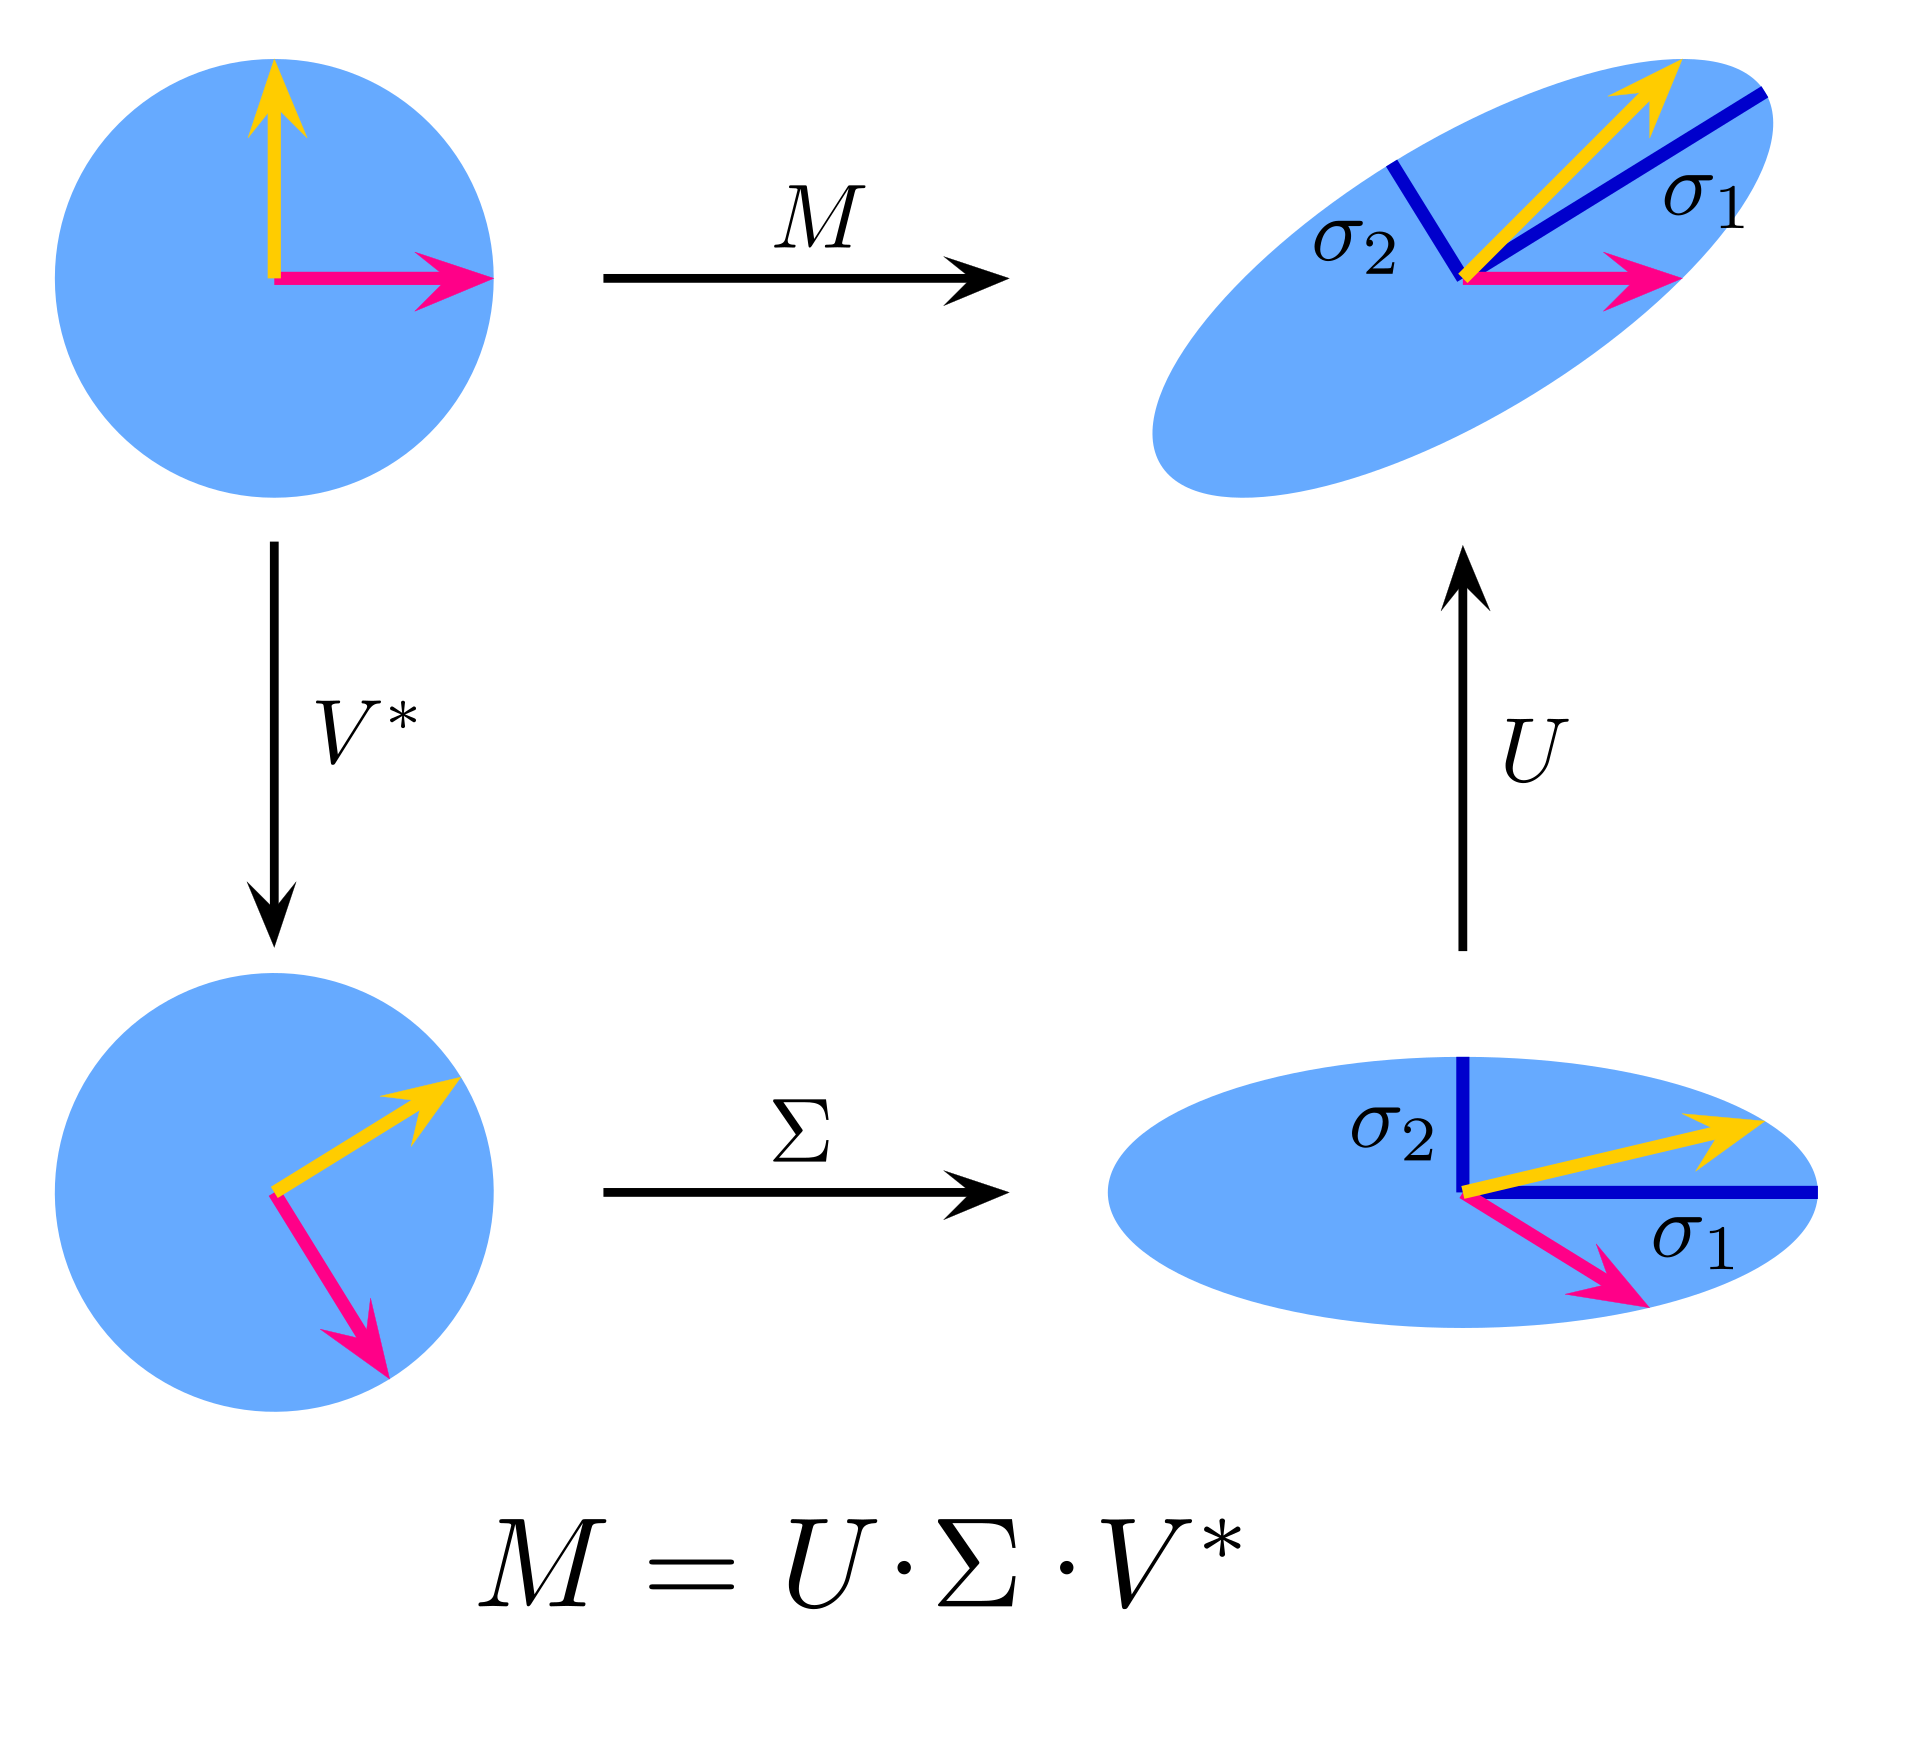
\includegraphics[width=0.4\textwidth]{lineareAlgebra/1920px-Singular-Value-Decomposition.svg.png}
    \caption*{Singulärwertzerlegung }
    \label{fig:svd}
\end{figure}

\subsubsection{Einfaches Berechnungsverfahren (über Eigenvektoren)}
\begin{enumerate}
    \item \(AA^T\) und \(A^TA\) bestimmen
    \item Für \glqq kleinere\dq Matrix aus 1) Eigenwerte \(\lambda_i\) bestimmen (char. Polynom)
    \item \(\Sigma\) mit \(diag(\sigma_1 \geq \sigma_2 \geq \hdots \geq \sigma_n)\) aufstellen; Singulärwerte \(\sigma_i = \sqrt{\lambda_i}\) auf Hauptdiagonalen; Rest \(=0\)
    \item \(U\) aufstellen: normierte Eigenvektoren für \(AA^T\) für alle \(\lambda_i\) bestimmen
    \item \(V\) aufstellen: normierte Eigenvektoren für \(A^TA\) für alle \(\lambda_i\) bestimmen; \(V^T\) bilden
\end{enumerate}



\subsubsection{Alternatives Berechnungsverfahren}

\begin{table}[H]
  \centering
  \begin{tabularx}{\textwidth}{X|l}
    %%%%%%%%%%%%%%%%%%%%%%%%%%%%%%%
    % 1. Form prüfen
    %%%%%%%%%%%%%%%%%%%%%%%%%%%%%%%
    \makecell[l]{\textbf{1. Form prüfen:} ist \(A\) \glqq hochkant\grqq? \\
        \(\rightarrow\) sonst aufwendiger zu lösen\\
        Umstellen zu \(A^T\) ist möglich, da\\
        \((A^T)^T = A\); d.h. \(A^T = V\Sigma^T U^T\)
    }
        &        
    \(A = \begin{pmatrix}       
        1 & 0 \\
        2 & 2 \\
        0 & 1
    \end{pmatrix}\)\\\\\hline

    %%%%%%%%%%%%%%%%%%%%%%%%%%%%%%%
    % 2. Eigenwerte bestimmen
    %%%%%%%%%%%%%%%%%%%%%%%%%%%%%%%
    \makecell[l]{\textbf{2. Eigenwerte von \(A^T A\) bestimmen} \\
        Eigenwerte (\(\geq 0\)) über \textit{Nullstellen char.}\\ \textit{Polynom} bestimmen,
        absteigend sortieren!
    }
        &
    \makecell[l]{            
        \(A^TA = \begin{pmatrix}       
            5 & 4 \\
            4 & 5
        \end{pmatrix}\) \\
        \(p_A(\lambda) = \det (A^T A - \lambda I) \overset{!}{=} 0\)\\
        \((5-\lambda)^2-16=0\)\\
        \(\lambda_1 = 9, \lambda_2 = 1\)
    }\\\\\hline

    %%%%%%%%%%%%%%%%%%%%%%%%%%%%%%%
    % 3. Sigma aufstellen
    %%%%%%%%%%%%%%%%%%%%%%%%%%%%%%%
    \makecell[l]{\textbf{3. \(\Sigma\) aufstellen} \\
        Diagonalmatrix mit \(\sigma_i=\sqrt[]{\lambda_i}\), Rest \(=0\)
    }
        &
    \makecell[l]{            
        \(\Sigma = \begin{pmatrix}       
            3 & 0 \\
            0 & 1 \\
            0 & 0
        \end{pmatrix}\)
    }\\\\\hline

    %%%%%%%%%%%%%%%%%%%%%%%%%%%%%%%
    % 4. Spaltenvektoren für V ermitteln
    %%%%%%%%%%%%%%%%%%%%%%%%%%%%%%%
    \makecell[l]{\textbf{4. Spaltenvektoren für \(V\) ermitteln} \\
        Eigenvektoren zu \(\lambda\) aus 2. bestimmen. Da \(A^TA\) symmetrisch\\
        ist \(\Rightarrow\) alle Eigenräume sind bereits orthogonal zueinander\\
        Wenn kein eindeutiges Ergebnis: ggf. \(v_1=1\) setzen.\\
        EV normieren und in Matrix \(V\) eintragen\\
        Für SVD: \(V^T\) bilden
    }
        &
    \makecell[l]{       
        \underline{für \(\lambda_1 = 9\):}\\     
        \(
            \left( 
            \begin{array}{cc|c}
                5 - 9 &  4 & 0\\
                4 & 5-9 & 0
            \end{array}
            \right)\Leftrightarrow 
        \)\\
        \(
            \left( 
            \begin{array}{cc|c}
                1 &  -1 & 0\\
                0 & 0 & 0
            \end{array}
            \right)\Rightarrow v_1^* = \begin{pmatrix}       
                1 \\
                1
            \end{pmatrix}
        \)\\
        \(v_1=\frac{v_1^*}{||v_1^*||} = \frac{1}{\sqrt{2}}\begin{pmatrix}
            1 \\
            1
        \end{pmatrix}\)\\\\
        \underline{für \(\lambda_2 = 1\):}\\ 
        \(\hdots\)\\
        \(v_2=\frac{v_2^*}{||v_2^*||} = \frac{1}{\sqrt{2}}\begin{pmatrix}
            -1 \\
            1
        \end{pmatrix}\)\\\\
        \(V = \frac{1}{\sqrt{2}}\begin{pmatrix}
            1 & -1 \\
            1 & 1
        \end{pmatrix}\)
    }\\\\\hline

    %%%%%%%%%%%%%%%%%%%%%%%%%%%%%%%
    % 5. U aufstellen
    %%%%%%%%%%%%%%%%%%%%%%%%%%%%%%%
    \makecell[l]{\textbf{5. \(U\) aufstellen} \\
        a) für vorhandene Singulärwerte:\\ \hspace*{1.5em}\(u_i = \frac{1}{\sigma_i}Av_i\)\\
        b) sonst: \(u_i\) so finden, dass \(u_i\) ONB sind\\
            \hspace*{1.5em}\(\rightarrow\) Kreuzprodukt (\(\mathbb{R}^3\))\\
            \hspace*{1.5em}\(\rightarrow\) Gram-Schmidt
    }
        &
    \makecell[l]{            
        \(u_1 = \frac{1}{3\sqrt{2}}\begin{pmatrix}
            1\\
            4\\
            1
        \end{pmatrix}\),
        \(u_2 = \frac{1}{\sqrt{2}}\begin{pmatrix}
            -1\\
            0\\
            1
        \end{pmatrix}\)\\
        b) \(u_3=u_1\times u_2 = \frac{1}{6}\begin{pmatrix}
            4\\
            -2\\
            4
        \end{pmatrix}\)\\
    }\\\\
    \end{tabularx}
\end{table}


\section{Optimierung}


\subsection{Konvexe Funktionen/Mengen}


Eine \emph{Menge} $G \subseteq \mathbb{R}^n$ heißt \emph{konvex}, wenn für alle $x, y \in G$ und $t \in [0, 1]$ gilt:
\begin{equation*}
t x + (1 - t) y \in G
\end{equation*}
D.h. die Verbindungsstrecke zwischen zwei Punkten der Menge liegt komplett in der Menge.
\\
\\
Eine \emph{Funktion} $f: \mathbb{R}^n \rightarrow \mathbb{R}$ heißt \emph{konvex} (\(\leq\)) bzw. \emph{strikt konvex} (\(<\)), wenn für alle $x, y \in \mathbb{R}^n$ und $t \in [0, 1]$ gilt:
\begin{equation*}
    f(t x + (1 - t) y) \leq t f(x) + (1 - t) f(y)
\end{equation*}

\underline{Vorgehensweise:}

\begin{enumerate}
    \item Hesse-Matrix (\(H_f(x)\), =symmetrisch) bestimmen:
            \(H_f(x) =
                \begin{pmatrix}
                    f_{xx} & f_{xy} \\
                    f_{yx} & f_{yy}
                \end{pmatrix}
            \)
    \item Definitheit bestimmen:
        \begin{enumerate}
            \item über \emph{Eigenwerte}
                \begin{itemize}
                    \item Nullstellen charakteristisches Polynom bestimmen (\(\rightarrow \) \ref{sec:charPolynom})
                    \item Interpretation:
                    \begin{itemize}
                        \item alle \(\lambda>0\rightarrow H_f(x)=\) pos. definit
                        \item alle \(\lambda\geq 0\rightarrow H_f(x)=\) pos. semidefinit 
                        \item alle \(\lambda<0\rightarrow H_f(x)=\) neg. definit 
                        \item alle \(\lambda\leq 0\rightarrow H_f(x)=\) neg. semidefinit 
                        \item \(\lambda\) positiv und negativ \(\rightarrow H_f(x)=\) indefinit
                    \end{itemize}
                \end{itemize}
            \item über \emph{Diagonaldominanz}: Ist \(H_f(x)\) Diagonaldominant und alle Diagonalelemente \(>0\), so ist \(H_f(x)\) positiv definit.\\
                \(\rightarrow \) für alle Zeilen: \(||\)Diagonalelement\(|| > \sum ||\)übrige Zeilenelemente\(||\) 
            \item \emph{Choleskyzerlegung} ist möglich \(= H_f(x)\) ist positiv definit
        \end{enumerate}
    \item Konvexität bestimmen:
        \begin{itemize}
            \item \(H_f(x)\) positiv definit \(\Leftrightarrow\) \(f\) strikt konvex
            \item \(H_f(x)\) positiv semidefinit \(\Leftrightarrow\) \(f\) konvex
            \item \(H_f(x)\) negativ definit \(\Leftrightarrow\) \(f\) strikt konvex
            \item \(H_f(x)\) negativ semidefinit \(\Leftrightarrow\) \(f\) konvex
        \end{itemize}
\end{enumerate}

\subsection{Optimierung ohne Nebenbedingungen}

\subsection{Optimierung ohne NB - Gradientenverfahren}
Beginnend an einer Stelle \(x_0\): 
\begin{enumerate}
\item Berechne Gradienten \(\nabla f(x_n)\) (im ersten Schritt mit \(x_0\))
\item Setze \(x_{n+1} = x_n - \alpha \nabla f(x_n), \;\;\;\; n \geq 0\) mit Schrittweite \(\alpha\)
\item Wiederhole Schritt 1 und 2 bis Abbruchkriterium erfüllt; \(x^* = x_k\)
\end{enumerate}

Approximation von \(\nabla f(x_0)\) durch \(\frac{f(x_n) - f(x_{n-1})}{x_n - x_{n-1}}\) möglich.

\subsubsection{Newton-Verfahren}

\subsection{Optimierung unter Nebenbedingungen}
Lagrangemultiplikatoren\\
Dualität\\
KKT-Bedingungen

\end{document}